
\section{Galactic Chemical Evolution Models}
\label{outflows:sec:gce}
We now construct GCE models to understand the origin of the radial age and
metallicity gradients characterized in~\S~\ref{outflows:sec:empirical}.
To this end, we construct models describing the Galaxy disk as a series of
one-zone models like those in Chapters~\ref{bursts} and~\ref{dga} and
multi-ring models like those in Chapters~\ref{migration} and~\ref{ohno}.
Though similar, the former does not incorporate mixing of stellar populations
while the latter does.
We also extend these models to incorporate radial gas
flows~\citep[e.g.,][]{Lacey1985, Bilitewski2012}.
We present models with numerical solutions predicted by multi-ring GCE models
of the Galactic disk accounting for both stellar migration and radial flows
(see~\S~\ref{outflows:sec:gce:multizone}), alongside which we develop an
analytic framework useful for qualitative interpretation
(see~\S~\ref{outflows:sec:gce:onezone:analytic}).

\subsection{One-Zone Models}
\label{outflows:sec:gce:onezone}
The fundamental assumption of one-zone GCE models is instantaneous
mixing of newly produced metals in the star-forming ISM.
In the presence of accretion, star formation, and outflows, the rate of
change of the ISM gas mass~$M_g$ can be expressed as
\begin{equation}\begin{split}
\dot{M}_g &= \dot{M}_\text{in} - \dot{M}_\star - \dot{M}_\text{out} +
\dot{M}_r
\\
&\approx \dot{M}_\text{in} - \dot{M}_\star(1 + \eta - r),
\label{outflows:eq:mdot-gas-noflow}
\end{split}\end{equation}
where~$\dot{M}_r$ is the rate of recycling from stellar envelopes being
returned back to the ISM.
Though this rate in detail depends on the initial mass function
\citep[IMF; e.g.,][]{Salpeter1955, Kroupa2001, Chabrier2003}, the
initial-final remnant mass relation~\citep[e.g.,][]{Kalirai2008}, and the
mass-lifetime relation~\citep[e.g.,][]{Larson1974, Maeder1989, Hurley2000},
to first order it is quite fast for young stellar populations but then
slows considerably due to the long lifetimes of low-mass stars.
As a result, it is sufficiently accurate for the purposes of analytic
approximations to take a constant value~$r$ that is returned immediately
after a stellar population forms ($r \approx +0.4$ for
a~\citealt{Kroupa2001} IMF; see discussion in~\citealt{Weinberg2017b}).
\par
We have also substituted the ``mass-loading factor''
$\eta \equiv \dot{M}_\text{out} / \dot{M}_\star$ into the above expression,
which is of central interest to this chapter.
This parameter describes how much ambient ISM is swept up and lost to outflows
due to feedback.
As discussed in~\S~\ref{outflows:sec:intro}, GCE models of the Milky Way
tend to fall into one of two categories: those with~$\eta = 0$ everywhere
\citep[e.g.,][]{Spitoni2021}, and those in which it grows exponentially
with radius~\citep[e.g.,][]{Johnson2021}.
\par
In the present chapter, we focus on the abundances of alpha and
iron-peak elements whose production is dominated by SNe
\citep[e.g.,][]{Johnson2019}.
We take O and Fe as the prototypical elements from these categories, though
we expect our GCE models to make similar predictions if we chose different
elements to compute abundances for.
The rate of change of the mass of some element~$x$ in the ISM can be
expressed as
\begin{equation}
\dot{M}_x = \ycc{$x$} \dot{M}_\star +
\yia{$x$} \langle \dot{M}_\star \rangle_\text{Ia} -
Z_x \dot{M}_\star \left(1 + \eta - r\right),
\label{outflows:eq:mdot-element-noflow}
\end{equation}
where~$Z_x$ is the abundance by mass of~$x$ in the ISM at a given moment in
time and~\ycc{$x$} and~\yia{$x$} are the population-averaged yields of~$x$
from core collapse supernovae (CCSNe) and Type Ia supernovae (SNe Ia),
respectively.
This parameterization assumes that all CCSNe yields are ejected immediately
following a stellar population's formation, which is valid as long as the
timescales of Galaxy evolution are significantly longer than the lifetimes
of massive stars.
Enrichment by SNe Ia is instead weighted by a delay-time distribution (DTD),
for which we retain the~$t^{-1.1}$ formalism from previous chapters as
suggested by comparisons of the cosmic SFH~\citep[e.g.,][]{Madau2017,
Driver2018} with volumetric SN Ia rates as a function of
redshift~\citep{Maoz2012a, Maoz2012b, Graur2013, Graur2014}.
\par
\citet{Weinberg2017b} demonstrate that the first-order details of the
enrichment history of alpha and iron-peak elements are established by
the mass-loading factor~$\eta$ and the star formation efficiency (SFE)
timescale~$\tau_\star \equiv M_g / \dot{M}_\star$ relating the
gas supply and the star formation rate (SFR).
The SFE timescale sets the position of the ``knee'' in the~\afe-\feh~plane,
while~$\eta$ controls the equilibrium abundance at which enrichment is
balanced by losses to outflows, which sets the end-point of the track.
The detailed form of the SFH has little impact, instead influencing how
stars distribute themselves along the track.
However, the detailed SFH has much more impact on the abundance evolution
in the~$\eta = 0$ scenario.
In this case, radial gas flows~\citep[e.g.,][]{Lacey1985}
also have a much stronger effect since the substantial sink term of
outflows is removed.
\par
To this end, we construct a parameterization for including the effects of
radial gas flows in one-zone GCE models.
We introduce the unitless coefficients~$\gamma_\flow$ and~$\mu_\text{flow}$
defined such that the rates of change of the gas supply and an element~$x$ due
to flows can be expressed in terms of the SFR and~$Z_x$ according to
\begin{subequations}\begin{align}
\dot{M}_{g,\flow} &= \dot{M}_\star \gamma_\flow
\label{outflows:eq:mdot-gas-flow}
\\
\dot{M}_{x,\flow} &= Z_x \dot{M}_\star \mu_\flow.
\label{outflows:eq:mdot-element-flow}
\end{align}\end{subequations}
Equations~\refp{outflows:eq:mdot-gas-noflow}
and~\refp{outflows:eq:mdot-element-noflow} then become
\begin{subequations}\begin{align}
\dot{M}_{g} &\rightarrow \dot{M}_\text{in} - \dot{M}_\star
\left(1 + \eta - r - \gamma_\flow\right)
\\
\dot{M}_x &\rightarrow \ycc{$x$} \dot{M}_\star +
\yia{$x$} \langle \dot{M}_\star \rangle_\text{Ia} -
Z_x \dot{M}_\star \left(1 + \eta - r - \mu_\flow\right).
\end{align}\end{subequations}
The most general forms of these flow coefficients are given by
\begin{subequations}\begin{align}
\gamma_\flow &\equiv -\tau_\star v_g \left[
\frac{1}{R} +
\frac{\partial \ln \Sigma_g}{\partial R} +
\frac{\partial \ln v_g}{\partial R}
\right]
\label{outflows:eq:gamma-flow-general}
\\
\mu_\flow &\equiv -\tau_\star v_g \left[
\frac{1}{R} + \frac{\partial \ln \Sigma_g}{\partial R} +
\frac{\partial \ln v_g}{\partial R} +
\frac{\partial \ln Z_x}{\partial R}
\right],
\label{outflows:eq:mu-flow-general}
\end{align}\end{subequations}
where~$v_g$ is the radial velocity of the ISM gas and~$\Sigma_g$ is its surface
density.
Though the ISM in nature has a distribution of radial velocities, this
parameterization assumes a single characteristic velocity at a given radius.
The bulk flow is generally directed inward (i.e.,~$v_g < 0$; hence the minus
signs), which arises due to the angular momentum of the disk being diluted by
freshly accreted material and falling toward the Galactic center
\citep[see discussion in, e.g.,][]{Bilitewski2012}.
These equalities should hold even when each of the quantities are allowed to be
arbitrary, continuous functions of time, but they are only as accurate as the
assumptions outlined in Appendix~\ref{outflows:sec:coefficients-derivation}.
We reserve detailed derivations of~$\gamma_\flow$ and~$\mu_\flow$ for
Appendix~\ref{outflows:sec:coefficients-derivation}, providing only
qualitative justification of their functional forms here.
\par
The linear dependence on~$v_g$ is expected.
As the flow velocity increases, its effect on enrichment rates and the gas
supply increases proportionally.
The dependence on the velocity profile is also intuitive.
For example, if the radial velocity slows as it falls due to, e.g., mixing with
higher density ISM on a less eccentric orbit, then its possible for material to
enter an annulus faster than it is leaving, leading to a ``pile-up.''
The linear dependence on~$\tau_\star$ arises because these rates are tied to
the local gas supply.
When multiplied by the SFR in equations~\refp{outflows:eq:mdot-gas-flow}
and~\refp{outflows:eq:mdot-element-flow},~$\dot{M}_\star \tau_\star$ becomes
$M_g$ by definition.
Both coefficients depend on fluctuations in the ISM surface density since any
variation thereof will affect how much gas is exchanged between neighboring
annuli.
The metal flow coefficient~$\mu_\flow$ additionally depends on the abundance
gradient for similar reasons.
For an inward flow, any given annulus will be replenished with less gas and
less metals from the next annulus at~$R + \Delta R$ if both decrease steeply
with radius.
Lastly, both coefficients have an explicit~$1 / R$ dependence on radius which
arises due to the change in area~$2 \pi R \Delta R$.
Though a pile-up can occur due to the radial velocity profile, this term
describes the inevitable pile-up near the Galactic center as the infalling
material converges.
\par
For a typical spiral galaxy like the Milky Way, the surface density of gas is
often described as an exponential
\begin{equation}
\Sigma_g \propto e^{-R / R_g},
\end{equation}
where~$R_g$ is some scale radius.
Similarly, abundance gradients are generally characterized as linear in [X/H],
which then translates to an exponential~$Z_x \propto e^{-R / R_x}$ in the
metal mass fraction.
Under these conditions, equations~\refp{outflows:eq:gamma-flow-general}
and~\refp{outflows:eq:mu-flow-general} become
\begin{subequations}\begin{align}
\gamma_\flow &\rightarrow -\tau_\star v_g
\left(\frac{1}{R} - \frac{1}{R_g}\right)
\label{outflows:eq:gamma-flow}
\\
\mu_\flow &\rightarrow -\tau_\star v_g
\left(\frac{1}{R} - \frac{1}{R_g} - \frac{1}{R_x}\right),
\label{outflows:eq:mu-flow}
\end{align}\end{subequations}
where~$R_x \equiv -(\grad{X}~\ln 10)^{-1}$ is the implied scale radius of the
abundance gradient in~$x$.
For~$\grad{x} \approx -0.06$ dex/kpc as found
in~\S~\ref{outflows:sec:empirical},~$R_x \approx 7.2$ kpc.
\par
In principle, both~$\gamma_\flow$ and~$\mu_\flow$ should be affected by changes
in~$\tau_\star$ with radius.
In particular, the low surface densities at large radii would imply inefficient
star formation~\citep[i.e., higher~$\tau_\star$; e.g.,][]{delosReyes2019,
Kennicutt2021}.
Combining a power-law scaling between~$\Sigma_g$ and the surface density of
star formation~$\dot{\Sigma}_\star$ with an exponential decline in~$\Sigma_g$
yields the following scaling of~$\tau_\star$ with radius:
\begin{equation}\begin{split}
\Sigma_g \tau_\star^{-1} &\propto \Sigma_g^N
\\
\implies \tau_\star &\propto \Sigma_g^{1 - N}
\\
\implies \tau_\star &= \tau_{\star,0} e^{(N - 1) R / R_g},
\end{split}\end{equation}
where~$\tau_{\star,0}$ is a normalizing constant specifying the efficiency of
star formation at~$R = 0$.
If~$N \approx 1.5$, consistent with the measurements of integrated SFRs and
surface densities in star forming spirals from~\citet{Kennicutt1998}, then
the scale radius that the SFE timescale increases over is exactly twice that
of the gas disk itself.
Based on the presence of the central molecular zone in the Milky Way
\citep[e.g.,][]{Morris1996, Dahmen1998, PiercePrice2000, Hatchfield2020} and
\citeauthor{Leroy2008}'s~\citeyearpar{Leroy2008} measurement that
$\tau_\star = 2$ Gyr for molecular gas,~$\tau_{\star,0} = 2$ Gyr is a
reasonable fiducial value.

\begin{figure*}
\centering
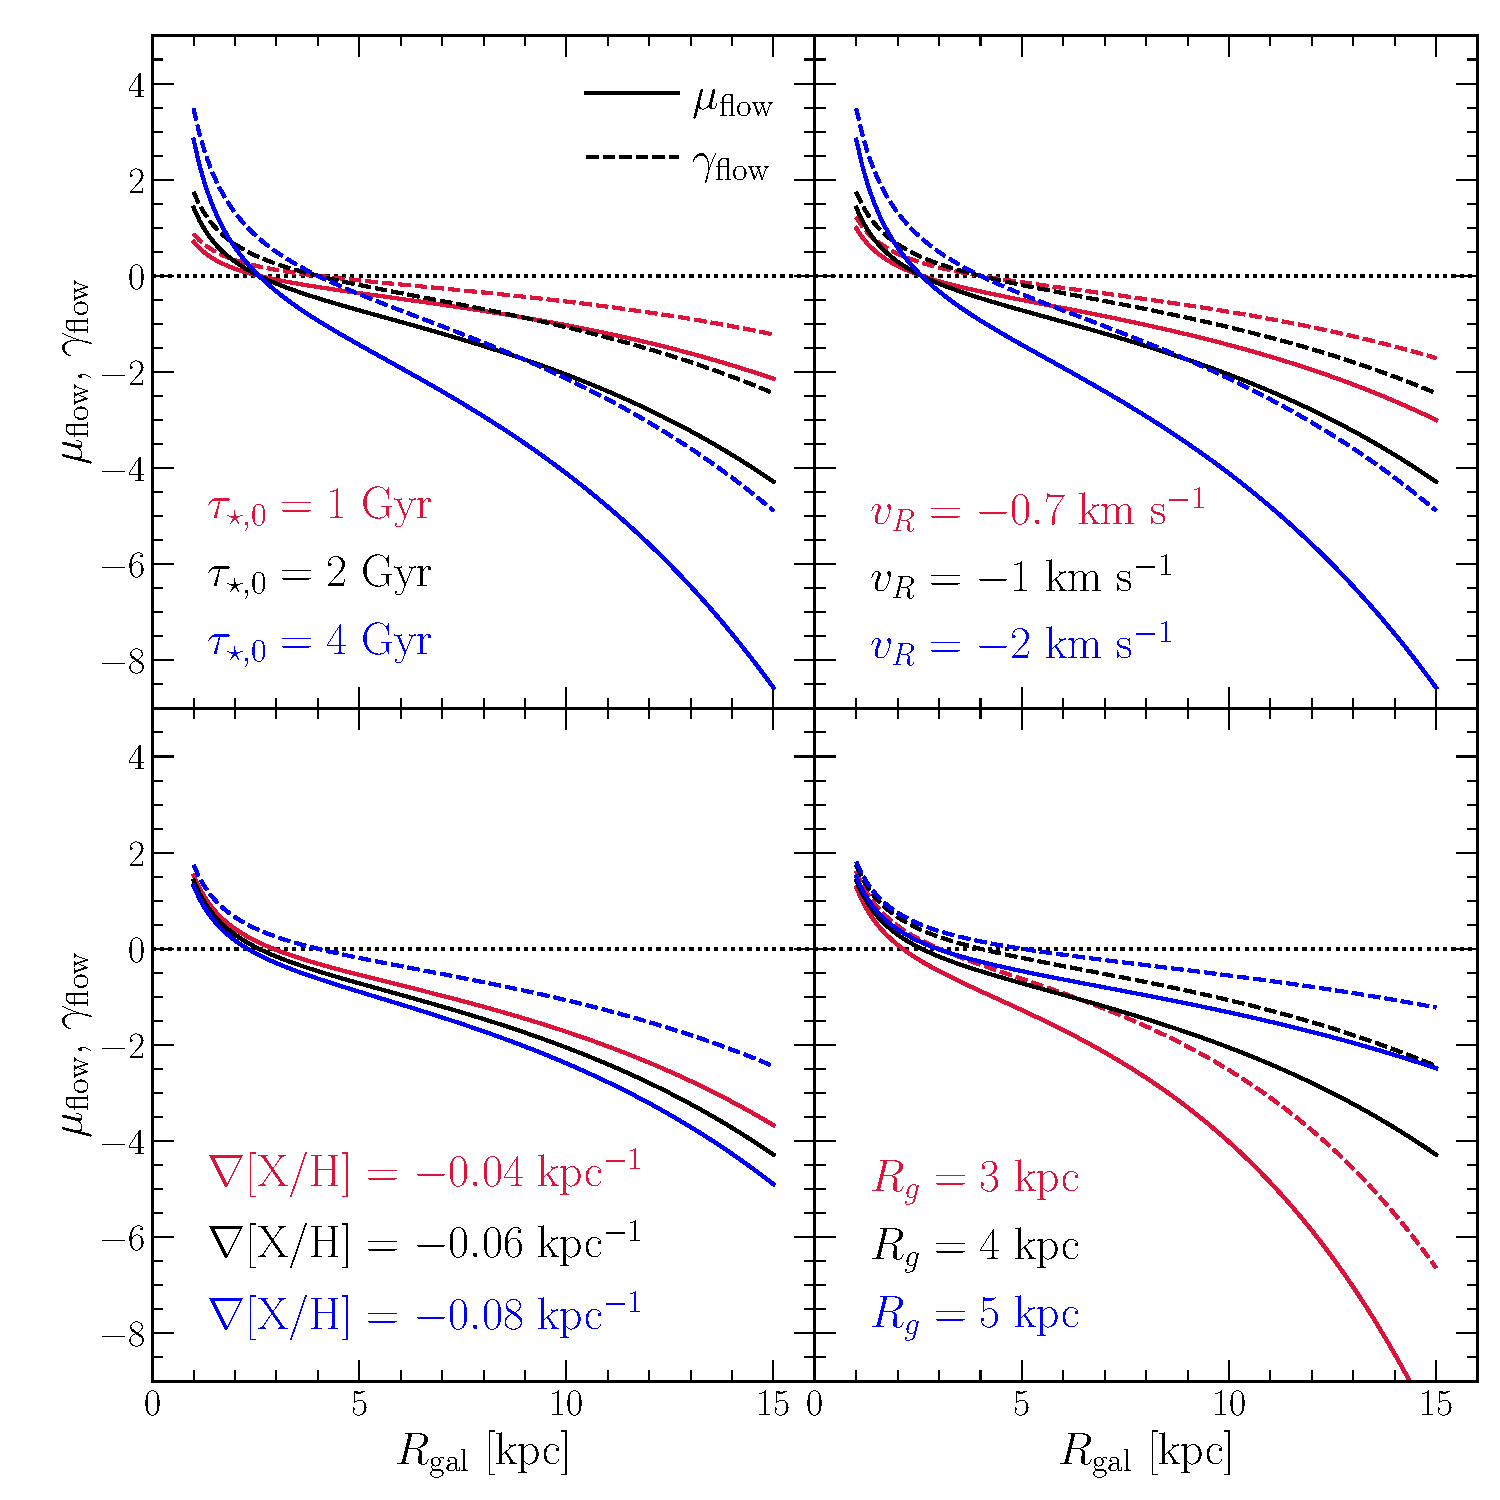
\includegraphics[scale = 0.5]{chapter7/muflow_gammaflow_vs_radius.pdf}
\caption{
The radial flow coefficients~$\mu_\flow$ (solid) and~$\gamma_\flow$ (dashed) as
functions of radius for different parameter choices.
Black lines correspond to the fiducial choice of
($\tau_{\star,0}$,~$v_g$,~\grad{X},~$R_g$) = (2 Gyr, 1 km s$^{-1}$,
$-0.06$ kpc$^{-1}$,~$4$ kpc) and are the same in all panels.
Each panel then shows variations in one of these four parameters according to
the legends in the lower right.
We also mark~$\mu_\flow$,~$\gamma_\flow = 0$ with a black dashed line, marking
the boundary between a radial flow acting as a source versus a sink of metals
and gas, respectively.
}
\label{outflows:fig:flow-coefficients-vs-radius}
\end{figure*}

Fig.~\ref{outflows:fig:flow-coefficients-vs-radius} shows~$\mu_\flow$
and~$\gamma_\flow$ as a function of radius for different parameter choices.
By definition, radial flows are a~\textit{source} of metals when~$\mu_\flow > 0$
and a~\textit{sink} when~$\mu_\flow < 0$; the same is true of the gas supply
with~$\gamma_\flow$.
In general, radial flows are a sink of both gas and metals across most of the
Galactic disk, becoming a source term only at radii better associated with the
bulge.
We expect this result to be generic as the negative sign arises due to the
difference between~$1 / R$, which varies, and~$1 / R_g + 1 / R_x$, which is
constant for a given parameter selection.
Flows are however a stronger sink for metals than gas under this
parameterization since, by definition,~$\mu_\flow = \gamma_\flow + \tau_\star
v_g / R_x$ and~$v_g < 0$.
Both~$\tau_{\star,0}$ and~$v_g$ are normalizing factors on the flow
coefficients, so they do not impact the radius at which~$\mu_\flow = 0$ or
$\gamma_\flow = 0$, but increases in their values make flows a stronger sink
where they are a sink and a stronger source where they are a source.
Changes in the slopes of gradients, either metallicity or gas surface density,
impact the flow rates in an intuitive manner: they are a stronger sink for more
sharply declining gradients as the mass or metallicity at~$R + \Delta R$ is
smaller in these cases.
Interestingly, the exact slope of the metallicity gradient~\grad{X} has minimal
impact on~$\mu_\flow$, potentially indicating that radial flows in turn have
minimal impact on abundance gradients.

\subsubsection{Analytic Solutions to Simple Cases}
\label{outflows:sec:gce:onezone:analytic}
Given a handful of simplifying assumptions, one-zone models often allow
analytic solutions to the abundance by mass~$Z_x \equiv M_x / M_g$ as a
function of time.
Under the approximation that the SN Ia DTD is a simple exponential followed by
some minimum delay,~\citet{Weinberg2017b} obtain solutions for~$Z_\text{O}$
and~$Z_\text{Fe}$ within the formalism of equations~\refp{outflows:eq:mdot-gas}
and~\refp{outflows:eq:mdot-element}.
With the additional approximation that~$\mu_\flow$ is constant in time, which
we expect to be accurate up to~$\sim$8 Gyr ago based on the results
of~\S~\ref{outflows:sec:empirical}, the derivation proceeds similarly under the
simple transformation~$1 + \eta - r \rightarrow 1 + \eta - r - \mu_\flow$.
We briefly discuss this extension of the~\citet{Weinberg2017b} results here and
refer readers to their~\S\S~2 and 3 for further details.
\par
The primary complication of the parameterization arises because
$\mu_\flow \neq \gamma_\flow$.
This inequality is a consequence of the radial metallicity gradient, which
lowers the metallicity of inward flowing gas.
% Fig.~\ref{outflows:fig:flow-coefficients-vs-radius} indicates that the amount
% of mass lost from a given~$\Delta R$ annulus at Galactocentric radii outside of
% the bulge over the course of some~$\Delta t$ timestep is replaced not only by
% less gas, but lower metallicity gas.
As a consequence, the~\textit{depletion time} of metals is shorter than that of
the bulk gas.
That is, in the absence of accretion (which would affect only the gas supply if
it is zero metallicity), metals spend less time than non-metals within a given
ISM fluid element before being incorporated into new stars or lost to an
outflow or the radial flow.
\par
These timescales are defined as
\begin{subequations}\begin{align}
\timescale{dep,g} &\equiv \frac{M_g}{
	\dot{M}_\star + \dot{M}_\text{out} - \dot{M}_r - \dot{M}_{g,\flow}
} = \frac{\tau_\star}{1 + \eta - r - \gamma_\flow}
\\
\timescale{dep,$x$} &\equiv \frac{M_x}{
	Z_x\left(\dot{M}_\star + \dot{M}_\text{out} - \dot{M}_r - \dot{M}_{x,\flow}
	\right)
} = \frac{\tau_\star}{1 + \eta - r - \mu_\flow},
\end{align}\end{subequations}
and both reduce to the~\citet{Weinberg2017b} form
$\timescale{dep} = \tau_\star / (1 + \eta - r)$ in the absence of a radial
flow (i.e.,~$v_g = 0 \implies \mu_\flow = \gamma_\flow = 0$).
In Appendix~\ref{outflows:sec:gce-supplement}, we demonstrate that their form
of~\timescale{dep} should be replaced with the metal depletion time as opposed
to the gas depletion time.
% A generic expression for~$\dot{Z}_x$ can be derived by differentiating
% $Z_x = M_x / (\dot{M}_\star \tau_\star)$ with time and substituting in
% equation~\refp{outflows:eq:mdot-element-flow}, carrying~$\mu_\flow$ as opposed
% to~$\gamma_\flow$ through the derivation.

{
\renewcommand{\arraystretch}{1.8}
\begin{table*}
\caption{
The SFHs we use in this analytic framework (left) and the implied functions of
time specifying the evolution toward chemical equilibrium (right; see equations
\ref{outflows:eq:z-o-eq} and~\ref{outflows:eq:fsfh-definition} and associated
discussion in~\S~\ref{outflows:sec:gce:onezone:analytic}).
}
\begin{tabularx}{\linewidth}{l @{\extracolsep{\fill}} r}
\hline
SFH Shape & $f_\text{sfh}$
\\
\hline
$e^{-t / \timescale{sfh}}$ &
$1 - e^{-t / \tau_\psi}$
\\
$te^{-t / \timescale{sfh}}$ &
$1 - \ddfrac{\tau_\psi}{t} \left(1 - e^{-t / \tau_\psi}\right)$
\\
$\left(1 - e^{-t / \timescale{rise}}\right) e^{-t / \timescale{sfh}}$ &
$\ddfrac{1}{1 - e^{-t / \timescale{rise}}} \left(
1 - e^{-t / \tau_\psi} -
\ddfrac{\timescale{rise}}{\timescale{rise} - \tau_\psi}
\left(e^{-t / \timescale{rise}} - e^{-t / \tau_\psi}\right)
\right)$
\\
\hline
\end{tabularx}
\label{outflows:tab:f-sfh-forms}
\end{table*}
}

As we are primarily interested in this analytic framework for qualitative
interpretation, we focus this component of our investigation on O.
This simplifies the parameterization as Fe abundances are additionally affected
by SN Ia enrichment (see discussion in~\S~X.Y.Z below), and the expressions
lend qualitative insight into the predicted Fe abundances anyway.
Applying our transformation to the~\citet{Weinberg2017b} formalism results in
the following expression for the equilibrium O abundance for the
linear-exponential and pure exponential SFHs:
\begin{equation}
Z_{\text{O,eq}} =
\frac{\ycc{O}}{1 + \eta - r - \mu_\flow - \tau_\star / \timescale{sfh}}.
\label{outflows:eq:z-o-eq}
\end{equation}
In Appendix~\ref{outflows:sec:gce-supplement}, we demonstrate that the
equilibrium abundance is the same for the ``inside-out'' SFH from
Chapter~\ref{migration}.
Of these three separate SFHs, the full time evolution of~$Z_x$ is given by
\begin{equation}
{Z}_\text{O}(t) = Z_\text{O,eq} f_\text{sfh}(t),
\label{outflows:eq:fsfh-definition}
\end{equation}
where~$f_\text{sfh}$ is some unitless function that depends on the SFH and
specifies the detailed evolution toward equilibrium with time.
Table~\ref{outflows:tab:f-sfh-forms} presents the time-dependence of these
SFHs and the associated forms of~$f_\text{sfh}$, where the timescale~$\tau_\psi$
is defined as 
\begin{equation}
\tau_\psi \equiv \left(
\frac{1 + \eta - r - \mu_\flow}{\tau_\star} - \frac{1}{\timescale{sfh}}
\right)^{-1}.
\label{outflows:eq:tau-psi-def}
\end{equation}
We also reserve the derivation of~$f_\text{sfh}$ for the inside-out SFH for
Appendix~\ref{outflows:sec:gce-supplement}.

\section{Multi-Ring Models}
\label{outflows:sec:gce:multizone}

